\section{Closed-loop issue with regular \ac{DeePC}}\label{sec:CL_ID_issue}




% ------------------------- Figure --------------------------
\begin{figure}
\begin{center}
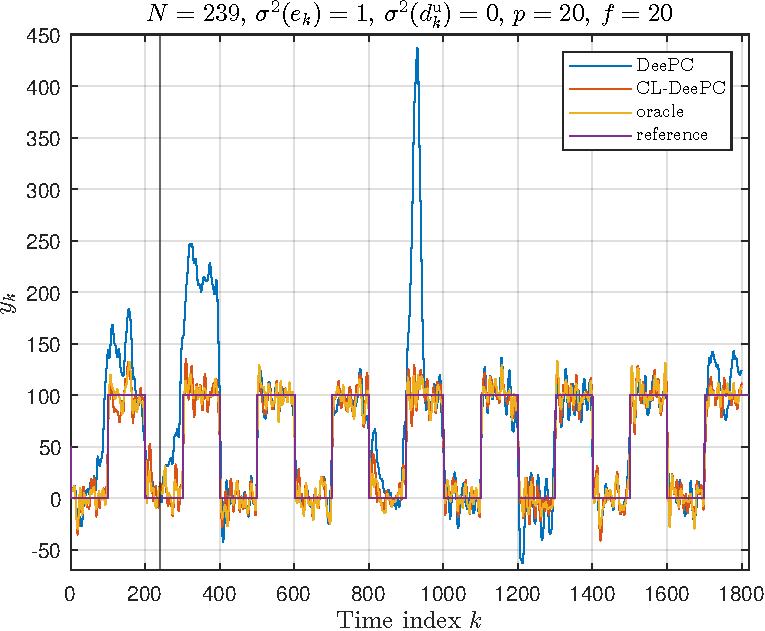
\includegraphics[width=\columnwidth]{results/figures/DeePC_CL_ID_issue_Re_1.mat_Nbar_239_p_20_f_20_Ru_1_Rdu_0_Q_100_R_0_dR_10.pdf}    % The printed column  
\caption{Reference tracking by adaptive \ac{DeePC} and \ac{CL-DeePC} using \ac{IVs} with $p=f=20$, $\bar{N}=539$, $Q=100$, $R=0$, $R^\Delta=10$, $|u_k-u_{k-1}|\leq3.75$, and $|u_k|\leq15$ for the system defined by \eqref{eq:SysFavoreel} with $\text{var}(e_k)=0.5$. %Both controllers are initialized by persistently exciting open-loop data. After $\bar{N}$ samples at the black vertical line, all used input-output data has been collected in closed-loop.
Unlike with \ac{CL-DeePC}, reference tracking by \ac{DeePC} deteriorates because of the closed-loop identification problem.}  % width is 8.4 cm.
\label{fig:CL_Problem_Solution}                                 % Size the figures 
\end{center}                                 % accordingly.
\end{figure}
% -----------------------------------------------------------